%\section{DEFINITION AND DCC INSERTION FLOW}
\section{FRAMEWORK}
\label{sec:DEF}
\begin{figure}
	\centering
	\includegraphics[width=0.9\columnwidth]{flow.png}
	\caption{DCC insertion flow}
	\label{fig:flow}
\end{figure}
\begin{comment}
\begin{figure}
	\centering
	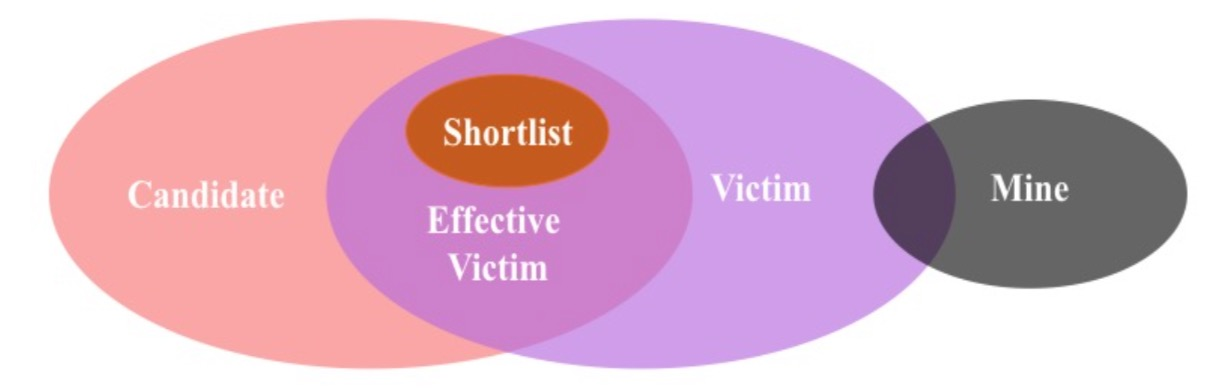
\includegraphics[width=0.9\columnwidth]{pathset.png}
	\caption{Classification of critical paths}
	\label{fig:set}
\end{figure}
\end{comment}
The overall flow of the proposed framework for DCC insertion/deployment is depicted in Figure~\ref{fig:flow}. The proposed framework focuses on the three issues: ($i$) Overhead minimization: Attacking all critical paths may be infeasible or may increase the used DCC count, which denotes the area overhead of the attack. Thus, the framework must filter/classify critical paths to make the attack successful and to minimize the DCC count. ($ii$) Process variations (PVs):  Because PVs impact the latencies of logic paths, it may degrade the lifetime accuracy of proposed Trojan. To be PV-aware, the above mentioned classification of critical paths considers the effect of PVs, where a model is introduced to consider the correlation of PVs and aging. ($iii$) Workload variation: Because users' workload highly impact the degradation of logic paths, the proposed framework must consider users' countless operational modes (i.e., workload). To be workload-aware, the problem of selecting target paths to be attacked is solved using the algorithms of \textbf{Minimum Domination Set}. Therefore, a graph is constructed according to the correlation and regression between critical paths. Note that, in the graph, a vertex represents a critical path, and an edge between two vertices (i.e., a pair of critical paths) denotes the correlation/regression between them. After target paths are determined, the problem of DCC insertion is transformed to a Boolean satisfiability formulation, which can be solved by existing SAT solvers such as miniSat. Finally, after the locations of DCC insertions are outputted from SAT solver, we estimate the circuit lifetime to evaluate the quality of our HTH attack with the impact of PVs.

%The section is organized as follows: Section~\ref{sec:DEF:CP} discusses the classification of critical paths, Section~\ref{\label{sec:shortlist}} discusses the PV-aware method, which considers the correlation of PVs and aging, and [subsection 3] introduces the SAT-based formulation of DCC insertion.
The section is organized as follows: Section~\ref{sec:DEF:CP} discusses the classification of critical paths and Section~\ref{sec:SAT} introduces the SAT-based formulation of DCC insertion/deployment.

\subsection{Classification of Critical Paths}
\label{sec:DEF:CP}
Given a critical path, the path is classified into three groups: \textit{Shortlist}, \textit{Candidate}, and \textit{Mine}, depending on the lifetime distribution of the path with DCC deployments on the associated clock network. Note that, the lifetime of a critical path is defined as when the timing violation occurs on the path. In addition, a DCC deployment results in an individual lifetime value of the critical path. Thus, given a critical path, numerous DCC deployments on the associated clock paths forms the lifetime distribution of the path. The lifetime distribution of the path is further analyzed with three lifetime intervals, which are defined as follows: $[0, n - \varepsilon]$, $[n - \varepsilon, n + \varepsilon]$, and $[n + \varepsilon, \infty]$, where $n$ is the expected circuit lifetime under the proposed HTH attack and $\varepsilon$ is mximum tolerable error. The lifetime distributions of the path in the three intervals determine the classification of the critical path. 
 
\begin{itemize}
	\item \textit{Candidate}: A critical path is defined as a candidate if there at least exists one DCC deployment, which leads the critical path to fail within $[n - \varepsilon, n + \varepsilon]$.
	\item \textit{Mine}: A critical path is defined as a mine if it satisfies the following conditions: ($i$) The path is not a candidate. That is, on the associated clock paths of the critical path, there is no DCC deployment to control the path lifetime within $[n - \varepsilon, n + \varepsilon]$. ($ii$) On the associated clock paths, there at least exists one DCC deployment, which leads the critical path to fail within $[0, n - \varepsilon]$, i.e., it lead the critical path to fail prematurely.
	\item \textit{Shortlist}:  Critical paths in \textit{shortlist} is the subset of \textit{Candidate}, which are selected as target paths to be attacked. Attacking such paths involves deploying DCCs on their associated clock paths.
\end{itemize}
%------- DSN 2018v -------------------------------------------------------------------------------------------------------------------------------
%Our proposed flow of DCC insertion is shown in Figure~\ref{fig:flow}. First, we read the data (e.g. circuit netlist, timing report, aging prediction parameters) and perform preprocessing. The detail about preprocessing will be described later. Then, a graph is constructed according to the correlation and regression between critical paths. In the graph, a vertex represents a critical path, and an edge between two vertices (i.e., a pair of critical paths) represents the correlation/regression between them. Afterwards, we choose some paths as our targets and transform our problem of DCC insertion based on SAT (Boolean Satisfiability), which can be solved by existing SAT solvers such as miniSat. Finally, we estimate the circuit lifetime after DCC insertion to evaluate the quality of our HTH attack.

%------- Definition -------------------------------------------------------------------------------------------------------------------------------
\begin{comment}
\textbf{\uline{Definition}}
\begin{itemize}
	\item $n$: Expected circuit lifetime under the proposed HTH attack based on DCC insertion. The unit is year.
	\item $\varepsilon$: Maximum tolerable error. The unit is year.
	\item \textit{Desired lifetime interval}: A desired interval of path/circuit lifetime under workload variations and statistical considerations of aging behavior among critical paths. Given $n$ and $\varepsilon$, the desired lifetime interval is $[ n - \varepsilon, n + \varepsilon]$.
\end{itemize}

%------- Terminology -----------------------------------------------------------------------------------------------------------------------------
\textbf{\uline{Terminology}}
\begin{itemize}
	\item \textit{Premature failure} denotes that a path leads to timing violations earlier than $n - \varepsilon$ years.
	\item \textit{Postmature failure} denotes that a path leads to timing violations later than $n + \varepsilon$ years.
	\item \textit{Proper failure} denotes that a path leads to timing violations within desired lifetime interval.
\end{itemize}

%------- Classification of DCC Placements --------------------------------------------------------------------------------------------------
\textbf{\uline{Classification of DCC Placements}}
\begin{itemize}
	\item \textit{Prematurely-failing DCC placement}: A kind of DCC placement which leads the critical path to premature failure.
	\item \textit{Properly-failing DCC placement}: A kind of DCC placement which leads the critical path to proper failure.
	\item \textit{Posmaturely-failing DCC placement}: A kind of DCC placement which leads the critical path to postmature failure.
	\item \textit{Illegal DCC placement (insertion)}: At most one DCC is allowed along a clock path from the clock source to a flip-flop. Placing more than one DCC along the same clock path is called illegal DCC placement.
\end{itemize}
%------- Classification of Critical Paths --------------------------------------------------------------------------------------------------
\textbf{\uline{Classification of Critical Paths}}
\begin{itemize}
	\item \textit{Candidate}: A critical path is defined as a candidate if there exists one properly-failing DCC placement.
	\item \textit{Shortlist}: A shortlist is a subset of candidates which are selected as target paths to be attacked. Attacking such paths involves placing DCCs on their associated clock paths.
	\item \textit{Mine}: A path is called a victim if one or more DCCs exist on its associated clock paths, as a result of attack on \textit{shortlist}.
	\item \textit{Effective victim}: A path is called an effective victim if it is a victim and the existing DCC(s) will lead the path to \textit{proper failure}.
\end{itemize}

Figure~\ref{fig:set} illustrates the relationship among those classification of critical paths. First, there is no intersection between candidate and mine. Second, the intersection between candidate and victim is effective victim. Third, shortlist is a subset of candidate; effective victim is a superset of shortlist, and so is victim. Moreover, victim and mine are likely to intersect because some paths in victim may belong to mine, and we have to ensure that these paths will not fail prematurely.
\end{comment}
%------- PV-Aware Methodology --------------------------------------------------------------------------------------------------
\subsection{Classification of Critical Paths Considering the Effect of PVs}
\label{sec:dcc_pv}
\begin{comment}
\begin{figure}
	\centering
	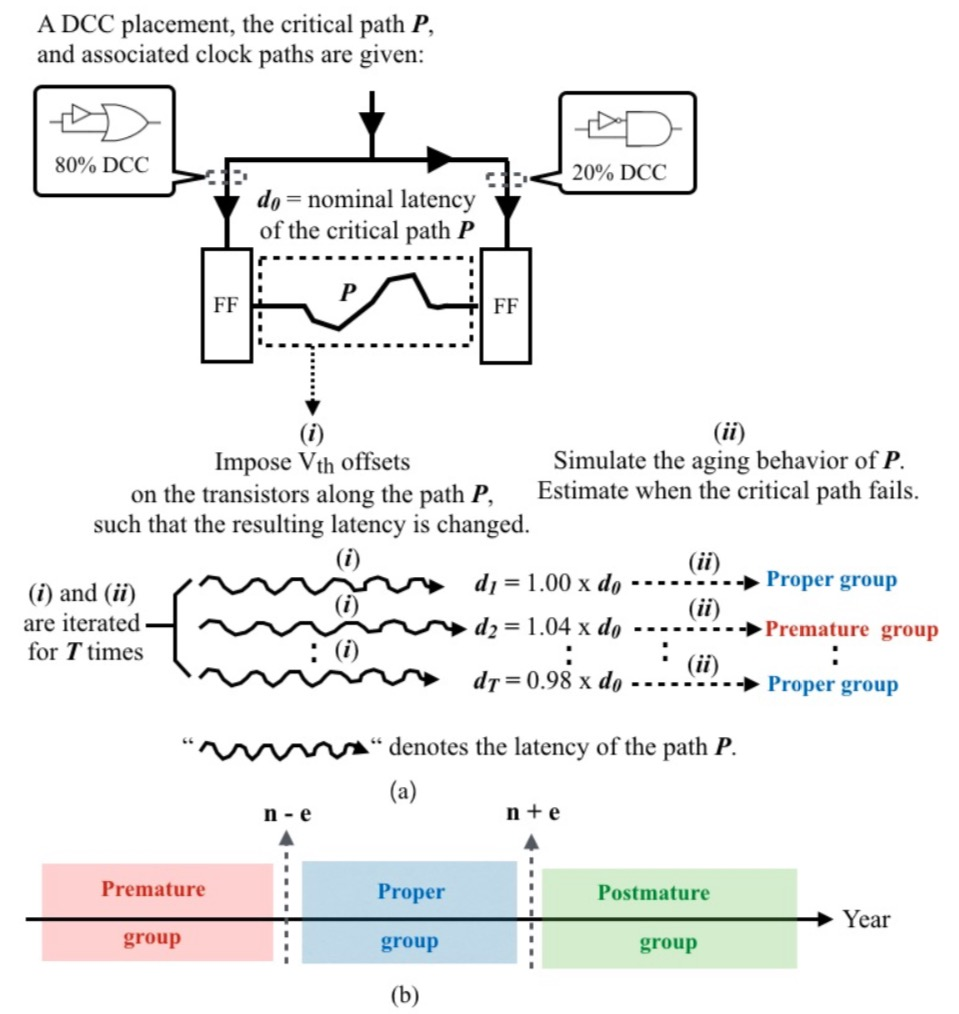
\includegraphics[width=0.9\columnwidth]{pvaware.png}
	\caption{Classification DCC placements considering process variation}
	\label{fig:pvaware}
\end{figure}
\end{comment}
As mentioned earlier, given a critical path, it is classified into the three groups, according to the path lifetime distribution within the three intervals. However, the lifetime estimation is impacted by PVs, degrading the lifetime accuracy of the proposed HTH attack. To make the proposed Trojan attack  PV-aware, the lifetime estimation considers the effect of PVs by Monte-Carlo simulation, which tests the PVs tolerability of the critical path, under each possible DCC deployment on the associated clock paths.                                                                                                                                                                                                                                                                                                                                                                                                                                                                                                                                                                                                                                                                                                                                                                                                                                                                 
%------- DSN 2018v --------------------------------------------------------------------------------------------------
\begin{comment}
Note that the classification of DCC placements introduced earlier is deterministic, i.e., unaware of process-induced timing variability when referring to timing violations. In this subsection, we include the influence of process variation (PV) when classifying DCC placements, such that the resulting attack is PV-aware.
The PV-aware method is depicted in Figure~\ref{fig:pvaware}(a). Given a DCC placement on the clock path associated with one critical path, we classify the DCC placement based on Monte-Carlo simulation with the following two procedures: (\textit{i}) Impose extra positive/negative V\textsubscript{th} offsets on the transistors along the critical path. Note that, the V\textsubscript{th} offsets follow a normal distribution, with the standard deviation of a specified value, which is usually set to 30mV. That is, 68\% of V\textsubscript{th} offsets of transistors reside between $\pm$ 30mV. (\textit{ii}) Then, a model, introduced in Section VI, is used to simulate the aging behavior of the critical path, such that we can estimate when the timing violation will occur. Note that, the model not only converts the V\textsubscript{th} offset to the delay shift of the transistor, but also considers the correlation of PV and BTI. The model will be explained in Section VI. Then, as illustrated in Fig. 6(a), the steps of (\textit{i}) and (\textit{ii}) are iterated for T times. Each iteration results in a time point, at which the critical path fails (i.e., timing violation occurs). Then, as shown in Figure~\ref{fig:pvaware}(b), the time points are categorized into 3 groups: premature group, proper group, and postmature group. Finally, we count the size of each group (i.e., the number of time points in the group). If the size of proper group is larger than a threshold, said H, the placement is classified as a properly-failing DCC placement. Otherwise, the sizes of the other two groups are compared. The larger one determines the classification of the DCC placement. For instance, if the size of
proper group is smaller than the threshold H, the sizes of premature group and postmature group are compared. Without the loss of generality, assume the size of postmature group is larger; then, the DCC placement is finally classified as postmaturely-failing one.
\end{comment}
%------- Shortlist selection --------------------------------------------------------------------------------------------------
\subsection{Selection of Target Paths (Shortlist) to be Attacked}
\label{sec:shortlist}
\begin{figure}
	\centering
	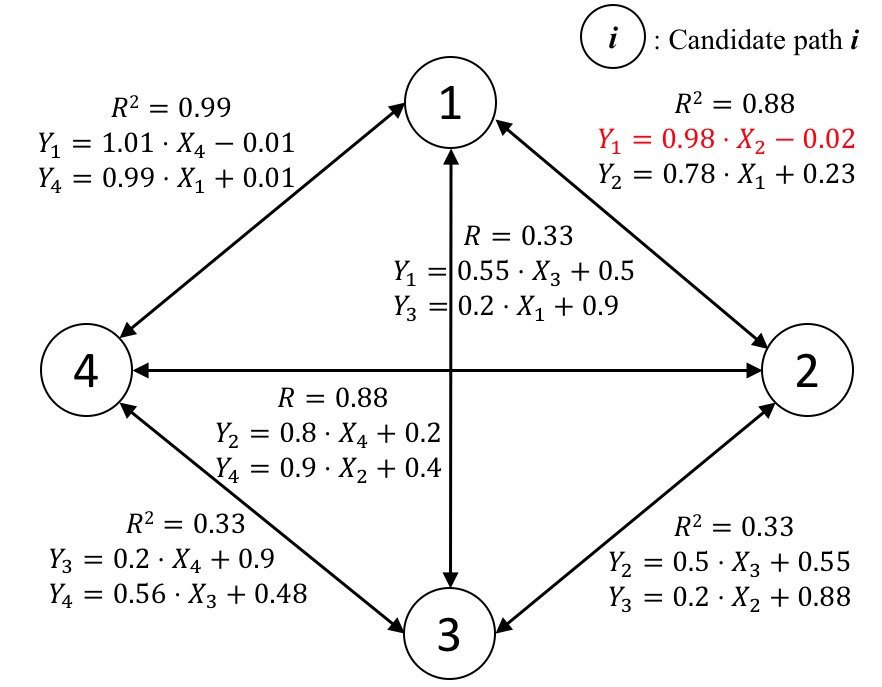
\includegraphics[width=0.9\columnwidth]{graph.png}
	\caption{Example of graph used in choosing targets}
	\label{fig:graph}
\end{figure}

If an attacked critical path always ages as estimated (i.e., under worst-case aging), a successful attack can be obtained just by inserting DCCs on its associated clock paths. How- ever, uncertainty of user-dependent operational modes (e.g., watching video, playing games) can influence/vary the aging behavior. Therefore, we must ensure that the attack will succeed under any operational mode. We make the following assumption, which will be used in Section [Undefined]:

\textit{"Every operational mode causes at least one candidate path to undergo worst-case aging."}

An operational mode, which causes one path to undergo worst-case aging, is called ?critical operational mode? of the path. Further, the union of critical operational modes of all candidate paths is equivalent to the universe of operational modes. Based on the assumption, attacking all candidates is a na�ve method to guarantee successful attack. Nevertheless, it is very costly and may be impossible.

Therefore, after observing the relationship among aging of paths, we find that the aging behaviors of many paths are highly correlated. If several paths are highly correlated in terms of aging behavior, one operational mode can lead all of them to age to a similar extent. Thus, we can simply attack one out of those highly correlated paths to cover multiple operational modes. For example, given two critical paths $A$ and $B$. Their critical operational modes are $O_{A}$ and $O_{B}$, respectively. Assume that $A$ and $B$ are highly correlated in terms of aging behavior. Because $A$ and $B$ age similarly/closely, $O_{A}$ causes $A$ to age in the worst-case and also causes $B$ to age severely. Consequently, even if we simply attack path $A$, not only $O_{A}$ but also $O_{B}$ can make the attack successful (premature failure of path $A$). This property helps reduce the number of targeted paths to be considered/formulated.
To choose the attack targets (shortlist), we transform the relationship of paths to a directed graph (also known as digraph). In Figure~\ref{fig:graph}, vertices represent candidates and arcs (i.e., directed edges) are correlation coefficients ($R^2$) and linear regression equations between each pair of vertices. Each arc has a regression equation, whose coefficients are obtained by running functional simulation. $X_{i}$ denotes the worst-case aging rate of path $i$, whose exact value will be introduced in Section [Undefined]. $Y_{j}$ denotes the aging rate of path $j$ predicted based on the linear regression equation. Consider the orange equation in Figure~\ref{fig:graph}:

\begin{equation*}
	\centering
	Y_{1} = 0.98 \cdot X_{2} - 0.02
\end{equation*}

Given the worst-case aging rate of vertex/path 2, $X_{2}$, the aging rate of vertex/path 1, $Y_{1}$, can be predicted as 0.98 multiplied by $X_{2}$ minus 0.02
Before the shortlist is determined by selecting a subset of candidates in the graph, we can simplify the graph by removing some arcs which indicate the relationships of weak aging correlation between pairs of paths.

The cost of our proposed HTHs is the count of inserted DCCs. In order to minimize the cost, we must select minimum-sized targets to cover all candidate paths, that is, to dominate all candidate paths in the digraph. This problem is similar to a classical digraph problem, \textbf{Minimum Dominating Set (MDS)}:

\textit{On digraph $G = (V, E)$, find a minimum-sized set of vertices $S \subseteq V$ such that $\forall y \notin S$, $\exists x \in S$, there exists an arc from $x$ to $y$. And we say that $y$ is dominated by $x$}.


%------- SAT  --------------------------------------------------------------------------------------------------
\begin{comment}
\subsection{Generation of SAT Formula}
\label{sec:SAT}
\begin{figure}
	\centering
	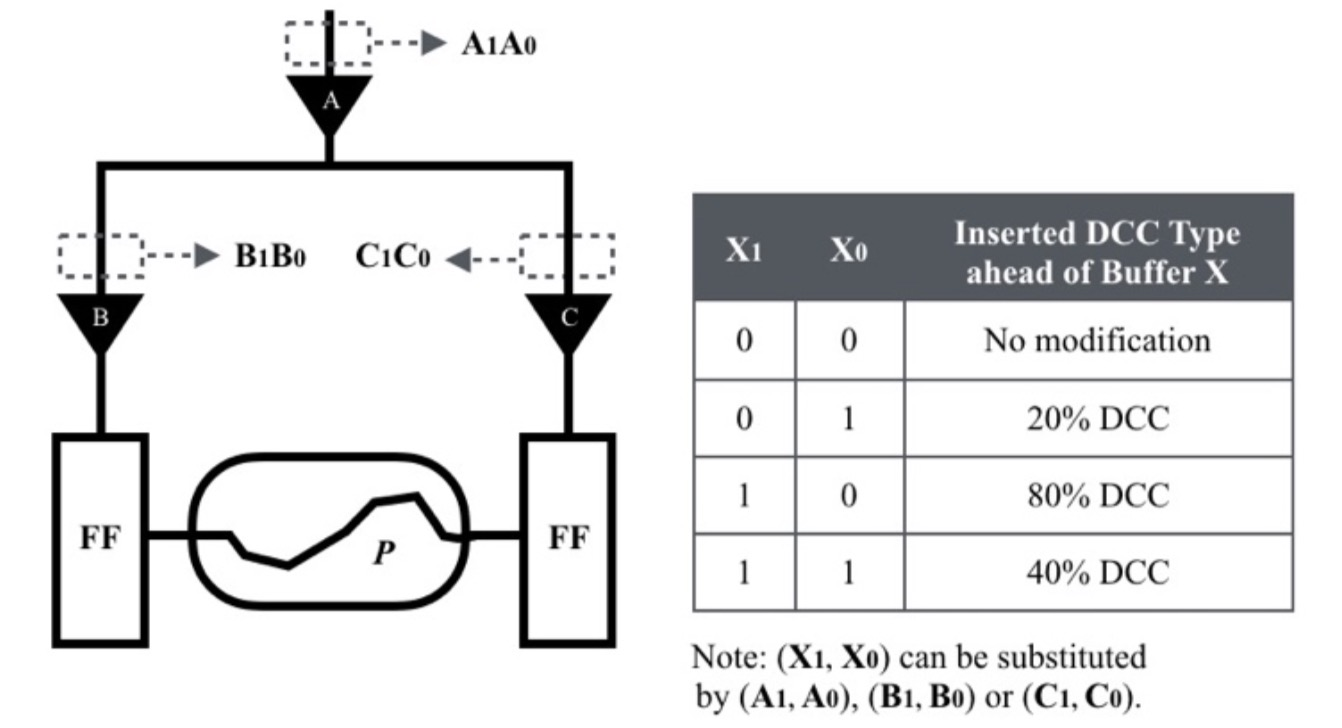
\includegraphics[width=0.9\columnwidth]{SAT.png}
	\caption{Introduction of SAT-formulation}
	\label{fig:sat}
\end{figure}
\begin{figure}
	\centering
	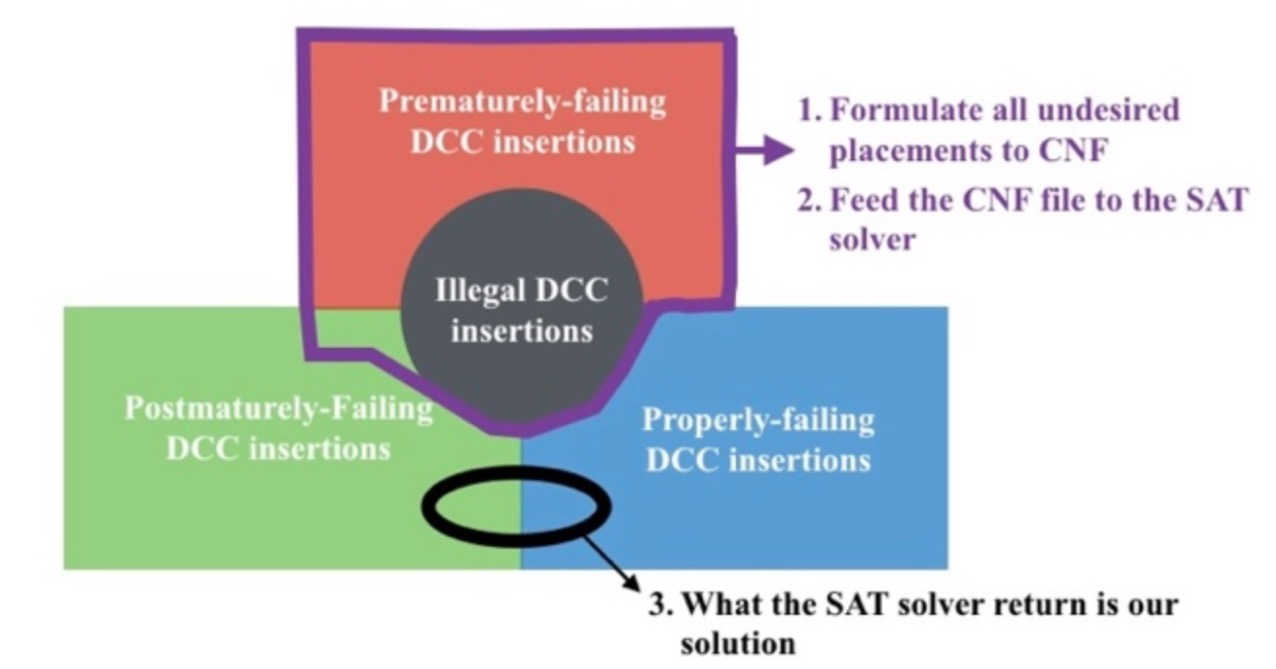
\includegraphics[width=0.9\columnwidth]{SAT_grp.png}
	\caption{SAT-formulation and relationship among 3 groups of DCC insertions}
	\label{fig:sat_grp}
\end{figure}
After the shortlist is determined, the problem is transformed into \textbf{Conjunctive Normal Form (CNF)}. That is, it is formulated as a \textbf{Boolean satisfiability (SAT)} problem. First, as shown in Figure~\ref{fig:sat}, each clock buffer is labeled by two Boolean variables to represent four types of DCCs (none, 20\%, 40\%, 80\%) inserted ahead of it. Next, the proposed formulation is based on the classification of critical paths:
\end{comment}

\subsection{SAT-based Problem Formulation and Encoding for DCC Deployment}
\label{sec:SAT}
\begin{comment}
\begin{figure}
	\centering
	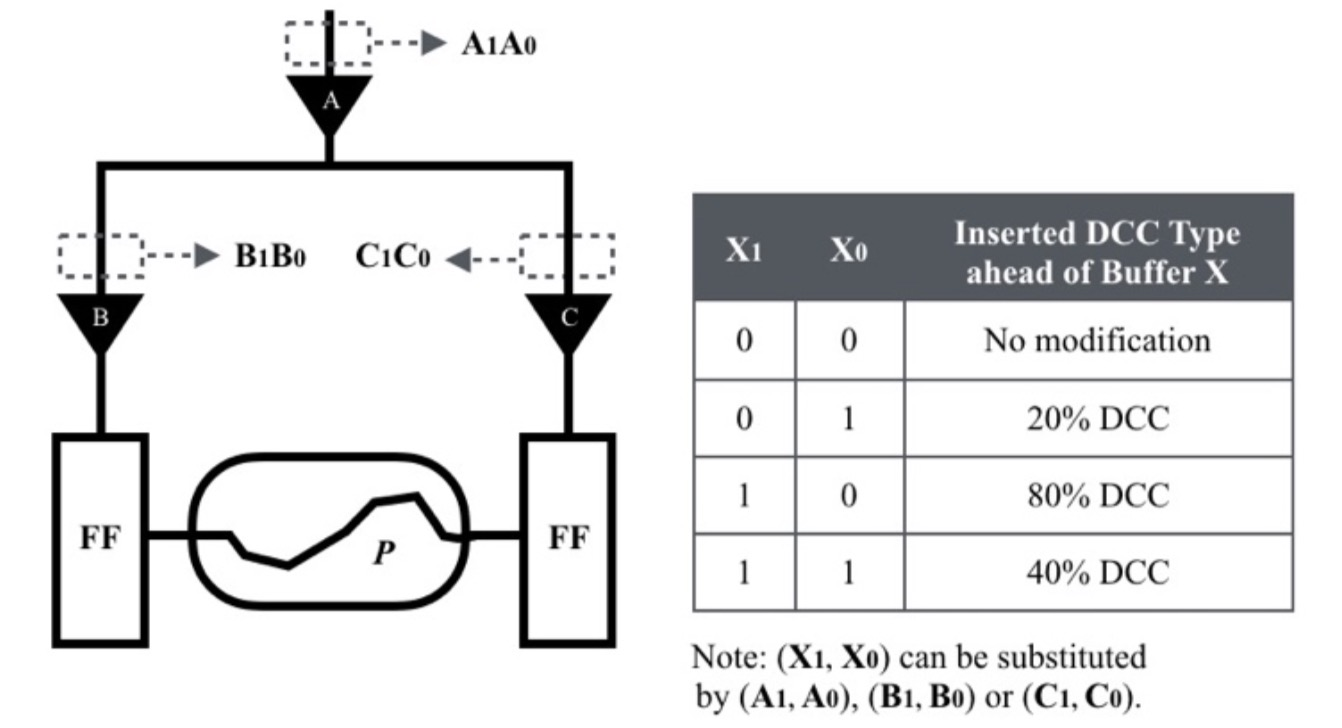
\includegraphics[width=0.9\columnwidth]{SAT.png}
	\caption{Introduction of SAT-formulation}
	\label{fig:sat}
\end{figure}
\begin{figure}
	\centering
	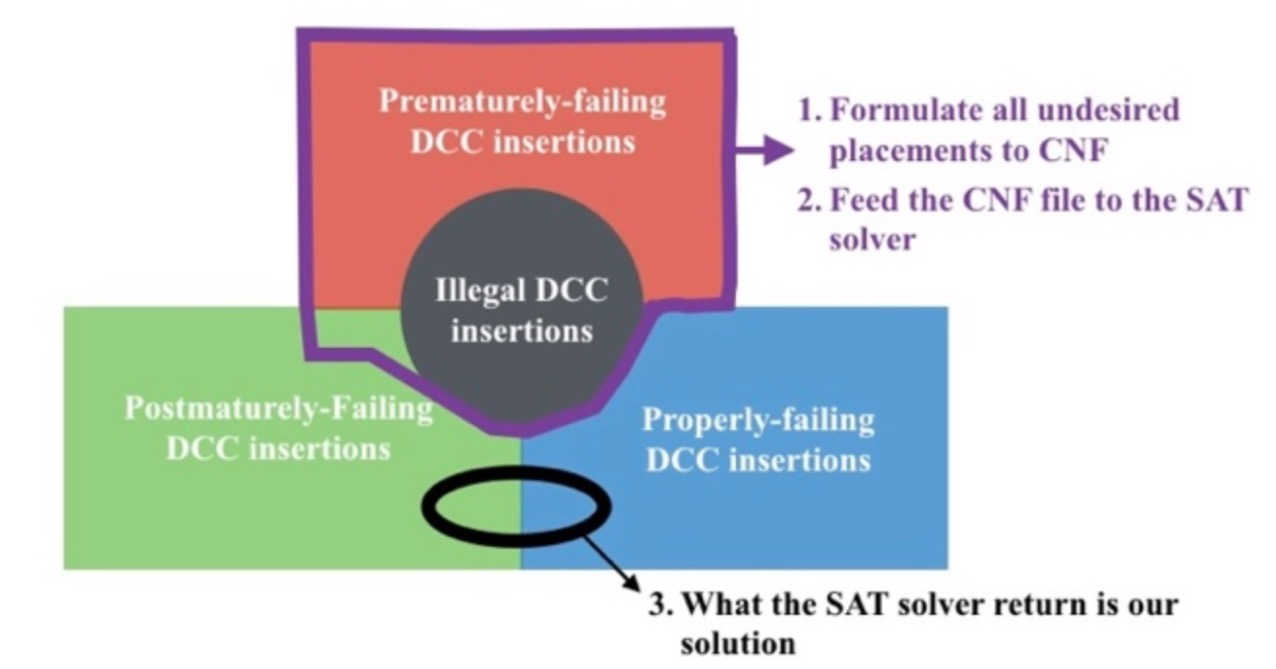
\includegraphics[width=0.9\columnwidth]{SAT_grp.png}
	\caption{SAT-formulation and relationship among 3 groups of DCC insertions}
	\label{fig:sat_grp}
\end{figure}
\end{comment}
\begin{figure*}[!ht]
    \centering
    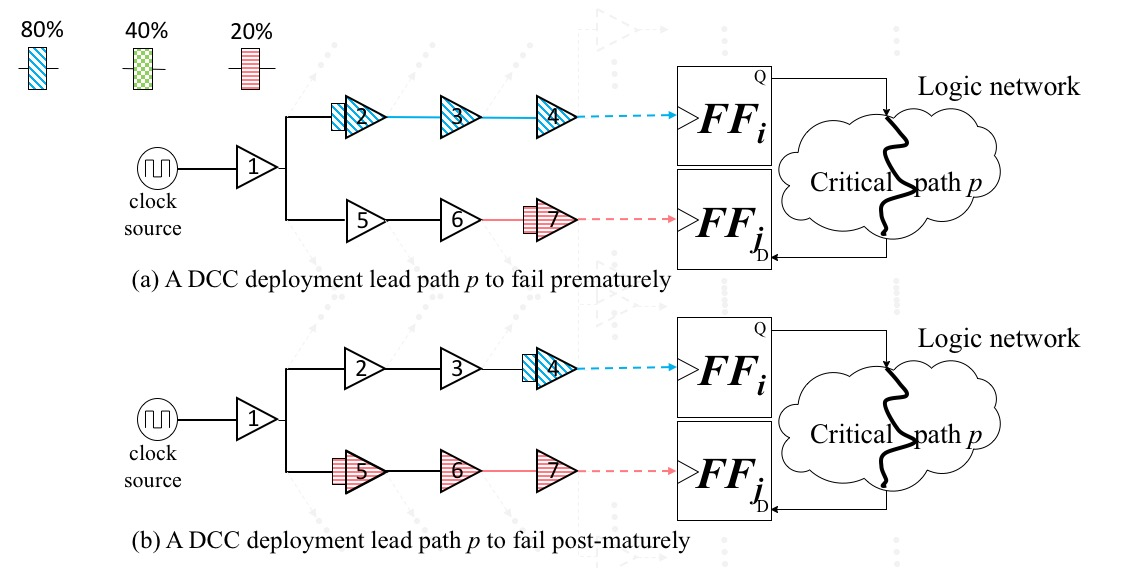
\includegraphics[width=1.1\columnwidth]{shortlist.png}
    \caption{Illustrative example for the proposed framework based on DCC deployment/insertion}
    \label{fig:shortlist}
\end{figure*}

After the shortlist (i.e., target paths to be attacked) is determined, the problem of DCC deployment on their associated clock paths is formulated as a \textbf{Boolean satisfiability (SAT)} problem. The key of the framework is to represent the problem in \textit{conjunctive normal form} (CNF). A CNF representation is a conjunction of one or more clauses, where each clause is a disjunction of one or more Boolean variables. Thus, DCC deployment/insertion needs to be encoded into Boolean representation before being transformed into a SAT-based formulation. Assume that a total of 3 types of DCCs can be chosen (i.e., 20\%, 40\%, and 80\% DCCs). Including the DCC-free case where no DCC is inserted, there are 4 possibilities of DCC insertion for each clock buffer. Given a clock buffer $p$, the four possibilities of DCC insertion at the input of buffer $p$ can be encoded as follows using two Boolean variables $B_{p,2}$ and $B_{p,1}$:

{\small
\begin{tabular}{ c c c }
   & DCC type & $\left\{B_{p,2},B_{p,1}\right\}$ \\
  (1)\quad & None & \{0,0\} \\
  (2)\quad & 20\% &  \{0,1\} \\
  (3)\quad & 40\% &  \{1,0\} \\
  (4)\quad & 80\% &  \{1,1\} \\
\end{tabular}}

In order to control the circuit lifetime near the expected circuit lifetime $n$, timing constraints of DCC deployments are involved in the SAT-based problem formulation, depending on the classification of critical paths.
\begin{enumerate}
	\item Paths in the shortlist (i.e., targets): On their associated clock paths, formulate all DCC deployments which lead the path to fail within $[ 0, n - \varepsilon]$ or within $[ n + \varepsilon, \infty]$. That is, the DCC deployments, which lead the path to fail prematurely and post-maturely, are formulated into CNF clauses, such that the SAT solver does not output the corresponding deployment in the result if the CNF is satisfiable.
	\item Other paths (paths not in the shortlist): On their associated clock paths, formulate all DCC deployments which lead the path to fail within $[ 0, n - \varepsilon]$. That is, the DCC deployments, which lead the path to fail prematurely, are formulated into CNF clauses, such that the SAT solver does not output the corresponding deployment in the result if the CNF is satisfiable.
\end{enumerate}

Consider the example in Figure~\ref{fig:shortlist} (a), where the 80\% and 20\% DCCs are inserted at the inputs of buffer 2 and 7, respectively. Assume that the critical path $p$ is in shortlist. If the DCC deployment will lead the path $p$ to fail prematurely (i.e., path fail within $[ 0, n - \varepsilon]$), then the following clause
\begin{gather*}
	\mbox{($A_{1} \lor A_{0} \lor \neg B_{1} \lor B_{0} \lor C_{1} \lor C_{0}$) } 
\end{gather*}
will be generated and added into CNF, such that the solver will not output the corresponding DCC deployment in the result if the CNF is satisfiable.

Consider the other example in Figure~\ref{fig:shortlist} (b), where the 80\% and 20\% DCCs are inserted at the inputs of buffer 4 and 5, respectively. Assume again that the critical path $p$ is in shortlist. If the DCC deployment will lead the path $p$ to fail post-maturely (i.e., path fail within $[ n + \varepsilon, \infty]$), then the following clause
\begin{gather*}
	\mbox{($A_{1} \lor A_{0} \lor B_{1} \lor B_{0} \lor C_{1} \lor \neg C_{0}$) } 
\end{gather*}
will be generated and added into CNF, such that the solver will not output the corresponding DCC deployment in the result if the CNF is satisfiable.

For SAT-based formulation, our proposed problem of DCC deployment is transformed into CNF clauses. The CNF clauses are solved by SAT solver such as MiniSat and we can find the locations and types of inserted DCCs by decoding the output from the solver.



